\documentclass{standalone}
\usepackage{tikz}
\usetikzlibrary{patterns, positioning}


\begin{document}
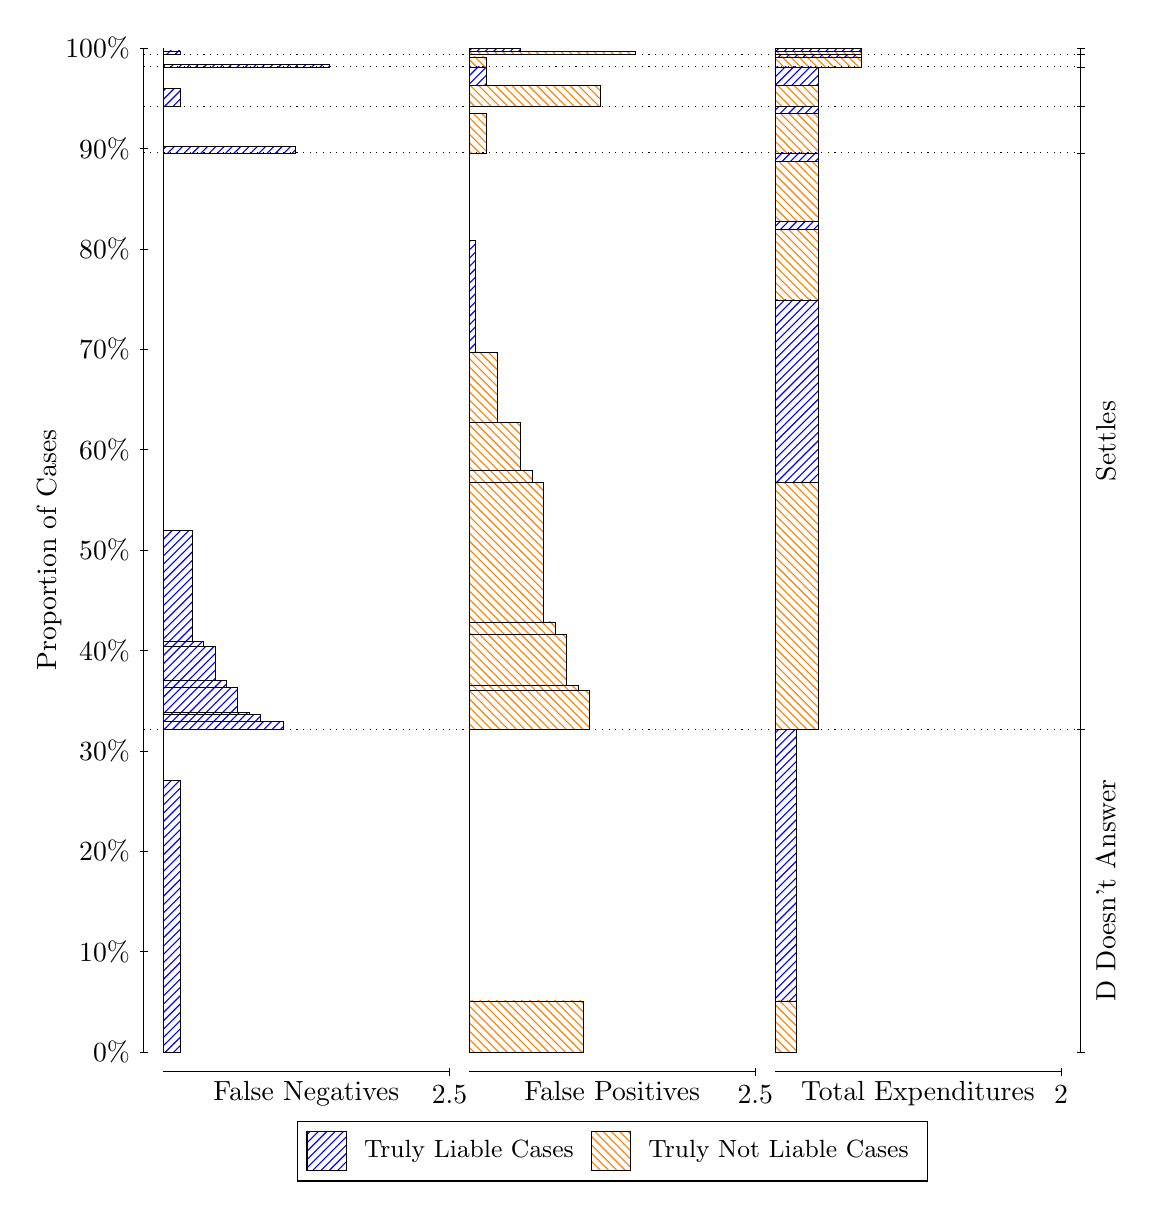
\begin{tikzpicture}
\draw[black, very thin] (1.5,1.75) -- (1.5,14.5);
\node[rotate=90, text=black, anchor=center] at (0.3, 8.125) {Proportion of Cases};
\draw[black, very thin] (1.45,1.75) -- (1.55,1.75);
\node[text=black, anchor=east] at (1.45, 1.75) {0\%};
\draw[black, very thin] (1.45,3.025) -- (1.55,3.025);
\node[text=black, anchor=east] at (1.45, 3.025) {10\%};
\draw[black, very thin] (1.45,4.3) -- (1.55,4.3);
\node[text=black, anchor=east] at (1.45, 4.3) {20\%};
\draw[black, very thin] (1.45,5.575) -- (1.55,5.575);
\node[text=black, anchor=east] at (1.45, 5.575) {30\%};
\draw[black, very thin] (1.45,6.85) -- (1.55,6.85);
\node[text=black, anchor=east] at (1.45, 6.85) {40\%};
\draw[black, very thin] (1.45,8.125) -- (1.55,8.125);
\node[text=black, anchor=east] at (1.45, 8.125) {50\%};
\draw[black, very thin] (1.45,9.4) -- (1.55,9.4);
\node[text=black, anchor=east] at (1.45, 9.4) {60\%};
\draw[black, very thin] (1.45,10.675) -- (1.55,10.675);
\node[text=black, anchor=east] at (1.45, 10.675) {70\%};
\draw[black, very thin] (1.45,11.95) -- (1.55,11.95);
\node[text=black, anchor=east] at (1.45, 11.95) {80\%};
\draw[black, very thin] (1.45,13.225) -- (1.55,13.225);
\node[text=black, anchor=east] at (1.45, 13.225) {90\%};
\draw[black, very thin] (1.45,14.5) -- (1.55,14.5);
\node[text=black, anchor=east] at (1.45, 14.5) {100\%};

\draw[black, very thin] (13.4,1.75) -- (13.4,14.5);
\draw[black, very thin] (13.35,1.75) -- (13.45,1.75);
\node[anchor=west] at (13.35, 1.75) {};
\draw[black, very thin] (13.35,5.8498) -- (13.45,5.8498);
\node[anchor=west] at (13.35, 5.8498) {};
\draw[black, very thin] (13.35,13.168) -- (13.45,13.168);
\node[anchor=west] at (13.35, 13.168) {};
\draw[black, very thin] (13.35,13.754) -- (13.45,13.754);
\node[anchor=west] at (13.35, 13.754) {};
\draw[black, very thin] (13.35,14.261) -- (13.45,14.261);
\node[anchor=west] at (13.35, 14.261) {};
\draw[black, very thin] (13.35,14.423) -- (13.45,14.423);
\node[anchor=west] at (13.35, 14.423) {};
\draw[black, very thin] (13.35,14.5) -- (13.45,14.5);
\node[anchor=west] at (13.35, 14.5) {};

\draw[black, very thin, pattern color=blue, pattern=north east lines] (1.75,1.75) rectangle (1.968,5.2016);
\draw[black, very thin, pattern color=orange, pattern=north west lines] (1.75,5.2016) rectangle (1.75,5.8498);
\draw[black, very thin, pattern color=blue, pattern=north east lines] (1.75,5.8498) rectangle (3.276,5.9498);
\draw[black, very thin, pattern color=blue, pattern=north east lines] (1.75,5.9498) rectangle (2.9853,6.0378);
\draw[black, very thin, pattern color=blue, pattern=north east lines] (1.75,6.0378) rectangle (2.84,6.0608);
\draw[black, very thin, pattern color=blue, pattern=north east lines] (1.75,6.0608) rectangle (2.6947,6.3823);
\draw[black, very thin, pattern color=blue, pattern=north east lines] (1.75,6.3823) rectangle (2.5493,6.4673);
\draw[black, very thin, pattern color=blue, pattern=north east lines] (1.75,6.4673) rectangle (2.404,6.8988);
\draw[black, very thin, pattern color=blue, pattern=north east lines] (1.75,6.8988) rectangle (2.2587,6.9604);
\draw[black, very thin, pattern color=blue, pattern=north east lines] (1.75,6.9604) rectangle (2.1133,8.379);
\draw[black, very thin, pattern color=orange, pattern=north west lines] (1.75,8.379) rectangle (1.75,13.168);
\draw[black, very thin, pattern color=blue, pattern=north east lines] (1.75,13.168) rectangle (3.4213,13.253);
\draw[black, very thin, pattern color=orange, pattern=north west lines] (1.75,13.253) rectangle (1.75,13.754);
\draw[black, very thin, pattern color=blue, pattern=north east lines] (1.75,13.754) rectangle (1.968,13.986);
\draw[black, very thin, pattern color=orange, pattern=north west lines] (1.75,13.986) rectangle (1.75,14.261);
\draw[black, very thin, pattern color=blue, pattern=north east lines] (1.75,14.261) rectangle (3.8573,14.297);
\draw[black, very thin, pattern color=orange, pattern=north west lines] (1.75,14.297) rectangle (1.75,14.423);
\draw[black, very thin, pattern color=blue, pattern=north east lines] (1.75,14.423) rectangle (1.968,14.464);
\draw[black, very thin, pattern color=orange, pattern=north west lines] (1.75,14.464) rectangle (1.75,14.5);
\draw[black, very thin, pattern color=orange, pattern=north west lines] (5.6333,1.75) rectangle (7.0867,2.3982);
\draw[black, very thin, pattern color=blue, pattern=north east lines] (5.6333,2.3982) rectangle (5.6333,5.8498);
\draw[black, very thin, pattern color=orange, pattern=north west lines] (5.6333,5.8498) rectangle (7.1593,6.3434);
\draw[black, very thin, pattern color=orange, pattern=north west lines] (5.6333,6.3434) rectangle (7.014,6.4101);
\draw[black, very thin, pattern color=orange, pattern=north west lines] (5.6333,6.4101) rectangle (6.8687,7.0533);
\draw[black, very thin, pattern color=orange, pattern=north west lines] (5.6333,7.0533) rectangle (6.7233,7.2118);
\draw[black, very thin, pattern color=orange, pattern=north west lines] (5.6333,7.2118) rectangle (6.578,8.9824);
\draw[black, very thin, pattern color=orange, pattern=north west lines] (5.6333,8.9824) rectangle (6.4327,9.1312);
\draw[black, very thin, pattern color=orange, pattern=north west lines] (5.6333,9.1312) rectangle (6.2873,9.7414);
\draw[black, very thin, pattern color=orange, pattern=north west lines] (5.6333,9.7414) rectangle (5.9967,10.639);
\draw[black, very thin, pattern color=blue, pattern=north east lines] (5.6333,10.639) rectangle (5.706,12.057);
\draw[black, very thin, pattern color=blue, pattern=north east lines] (5.6333,12.057) rectangle (5.6333,13.168);
\draw[black, very thin, pattern color=orange, pattern=north west lines] (5.6333,13.168) rectangle (5.8513,13.669);
\draw[black, very thin, pattern color=blue, pattern=north east lines] (5.6333,13.669) rectangle (5.6333,13.754);
\draw[black, very thin, pattern color=orange, pattern=north west lines] (5.6333,13.754) rectangle (7.3047,14.03);
\draw[black, very thin, pattern color=blue, pattern=north east lines] (5.6333,14.03) rectangle (5.8513,14.261);
\draw[black, very thin, pattern color=orange, pattern=north west lines] (5.6333,14.261) rectangle (5.8513,14.387);
\draw[black, very thin, pattern color=blue, pattern=north east lines] (5.6333,14.387) rectangle (5.6333,14.423);
\draw[black, very thin, pattern color=orange, pattern=north west lines] (5.6333,14.423) rectangle (7.7407,14.458);
\draw[black, very thin, pattern color=blue, pattern=north east lines] (5.6333,14.458) rectangle (6.2873,14.5);
\draw[black, very thin, pattern color=orange, pattern=north west lines] (9.5167,1.75) rectangle (9.7892,2.3982);
\draw[black, very thin, pattern color=blue, pattern=north east lines] (9.5167,2.3982) rectangle (9.7892,5.8498);
\draw[black, very thin, pattern color=orange, pattern=north west lines] (9.5167,5.8498) rectangle (10.062,8.9824);
\draw[black, very thin, pattern color=blue, pattern=north east lines] (9.5167,8.9824) rectangle (10.062,11.3);
\draw[black, very thin, pattern color=orange, pattern=north west lines] (9.5167,11.3) rectangle (10.062,12.198);
\draw[black, very thin, pattern color=blue, pattern=north east lines] (9.5167,12.198) rectangle (10.062,12.298);
\draw[black, very thin, pattern color=orange, pattern=north west lines] (9.5167,12.298) rectangle (10.062,13.057);
\draw[black, very thin, pattern color=blue, pattern=north east lines] (9.5167,13.057) rectangle (10.062,13.168);
\draw[black, very thin, pattern color=orange, pattern=north west lines] (9.5167,13.168) rectangle (10.062,13.669);
\draw[black, very thin, pattern color=blue, pattern=north east lines] (9.5167,13.669) rectangle (10.062,13.754);
\draw[black, very thin, pattern color=orange, pattern=north west lines] (9.5167,13.754) rectangle (10.062,14.03);
\draw[black, very thin, pattern color=blue, pattern=north east lines] (9.5167,14.03) rectangle (10.062,14.261);
\draw[black, very thin, pattern color=orange, pattern=north west lines] (9.5167,14.261) rectangle (10.607,14.387);
\draw[black, very thin, pattern color=blue, pattern=north east lines] (9.5167,14.387) rectangle (10.607,14.423);
\draw[black, very thin, pattern color=orange, pattern=north west lines] (9.5167,14.423) rectangle (10.607,14.458);
\draw[black, very thin, pattern color=blue, pattern=north east lines] (9.5167,14.458) rectangle (10.607,14.5);
\draw[black, dotted] (1.5,5.8498) -- (13.4,5.8498);
\draw[black, dotted] (1.5,13.168) -- (13.4,13.168);
\draw[black, dotted] (1.5,13.754) -- (13.4,13.754);
\draw[black, dotted] (1.5,14.261) -- (13.4,14.261);
\draw[black, dotted] (1.5,14.423) -- (13.4,14.423);
\draw[black, very thin] (1.75,1.5) -- (5.3833,1.5);
\node[text=black, anchor=north] at (3.5667, 1.5) {False Negatives};
\draw[black, very thin] (5.3833,1.45) -- (5.3833,1.55);
\node[text=black, anchor=north] at (5.3833, 1.45) {2.5};

\draw[black, very thin] (5.6333,1.5) -- (9.2667,1.5);
\node[text=black, anchor=north] at (7.45, 1.5) {False Positives};
\draw[black, very thin] (9.2667,1.45) -- (9.2667,1.55);
\node[text=black, anchor=north] at (9.2667, 1.45) {2.5};

\draw[black, very thin] (9.5167,1.5) -- (13.15,1.5);
\node[text=black, anchor=north] at (11.333, 1.5) {Total Expenditures};
\draw[black, very thin] (13.15,1.45) -- (13.15,1.55);
\node[text=black, anchor=north] at (13.15, 1.45) {2};

\node[text=black, centered, rotate=90] at (13.72, 3.7999) {D Doesn't Answer};
\node[text=black, centered, rotate=90] at (13.72, 9.5089) {Settles};





\draw (7.449999999999999,1.5) node[draw=none] (baseCoordinate) {};
\begin{scope}[align=center]
        \matrix[scale=0.5, draw=black, below=0.5cm of baseCoordinate, nodes={draw}, column sep=0.1cm]{
            \node[rectangle, draw, minimum width=0.5cm, minimum height=0.5cm, pattern color=blue, pattern=north east lines] {}; &
            \node[draw=none, font=\small, text=black] (B) {Truly Liable Cases}; &
            \node[rectangle, draw, minimum width=0.5cm, minimum height=0.5cm, pattern color=orange, pattern=north west lines] {}; &
            \node[draw=none, font=\small, text=black] (B) {Truly Not Liable Cases}; \\
            };
\end{scope}

\end{tikzpicture}
\end{document}